
\chapter{روش پیشنهادی و پیاده‌سازی}
\label{ch:method}

این فصل، ساختار سامانه و روش ساخت داده و طراحی آزمایش‌ها را شرح می‌دهد.
ترتیب مطالب چنین است: نخست تلاش اولیه و درسی که از آن گرفته شد؛ سپس
زنجیره ساخت مجموعه داده؛ آنگاه معماری سامانه آبشاری تحویل‌شده و ماژول
تشخیص وقفه و بستر انتقال تمام‌دوطرفه؛ سپس طراحی آزمایش‌های مسیر مستقیم؛ و
در پایان روش کاری شواهد‌محوری که چارچوب همه ارزیابی‌های فصل بعد است.

\section{تلاش اولیه و بازنگری در معماری}
\label{sec:early-attempt}

نخستین پیاده‌سازی پروژه بر پایه معماری \en{LLaMA-Omni2} بنا شد: یک کدگذار
گفتاری منجمد \en{Whisper}، یک لایه تصویرگر آموزش‌پذیر، یک مدل زبانی
\en{Qwen2.5-0.5B}~\cite{qwen2025qwen25} با آداپتر \en{LoRA}، و سرهای جداگانه برای بازشناسی و
تولید نشانه‌های گفتاری. این مصنوع آموزش دید و زیان آن کاهش یافت.

یک ممیزی درونی کد پیش از هرگونه گزارش نتیجه، سه اشکال بنیادی را آشکار کرد
که ثبت آن‌ها برای صداقت روشمند این نوشتار ضروری است:

\begin{itemize}
\item مدل زبانی در تابع پیش‌رو مشارکت نداشت؛ بنابراین آنچه آموزش می‌دید یک
      شبکه نگاشت صوتی بود و نه یک مدل زبانی گفت‌وگو‌محور.
\item هدف بازشناسی از درهم‌سازی‌های تصادفی‌شده در هر فرایند استفاده می‌کرد و
      در نتیجه برچسب‌های آموزشی میان اجراها ناپایدار بودند.
\item هدف تولید گفتار، «بازسازی همان اظهار ورودی» بود و نه تولید یک
      پاسخ گفت‌وگویی؛ و برای شنیدن خروجی، موتور گفتاری بیرونی مسیر مصنوع
      آموخته‌شده را دور می‌زد.

\end{itemize}

نتیجه‌گیری این ممیزی صریح بود: آن مصنوع یک مدل گفتار‌به‌گفتار نبود و
نمی‌توانست به‌عنوان چنین چیزی گزارش شود. این تجربه دو تصمیم تعیین‌کننده را
رقم زد. نخست، سرویس‌دهی سامانه به‌طور کامل به یک زنجیره آبشاری با مؤلفه‌های
واقعی و قابل آزمون منتقل شد. دوم، برای مسیر مستقیم تنها مدلی پذیرفته شد
که «آموزش‌دهنده رسمی» داشته باشد، تا هدف آموزشی و زنجیره داده به‌جای
بازنویسی محلی، از سوی سازندگان مدل تعیین شود. این دو تصمیم، شکل نهایی
پروژه را ساختند.

\section{ساخت مجموعه داده مکالمه فارسی}
\label{sec:data}

\subsection{منبع و راهبرد}

از آنجا که پیکره عمومی فارسی با برچسب وقفه در دسترس نبود
(بخش~\ref{sec:persian-resources})، مجموعه داده این پروژه از یک آرشیو داخلی
محتوای گفتاری فارسی مشتق شد. این آرشیو شامل برنامه‌های گفت‌وگویی بلند از
چهار کانال با سبک‌های متفاوت است. استفاده پژوهشی داخلی از این منابع با
تأیید استاد راهنما ثبت شده است؛ این تأیید مجوز بازنشر صوت یا زیرنویس خام
نیست و هیچ داده محدودشده‌ای در مخزن کد قرار نگرفته است.

نکته روشمندی که در میانه کار اصلاح شد ارزش ثبت دارد. در طرح نخست، برچسب
متنی هر بازه با اجرای مجدد سرویس بازشناسی گفتار تولید می‌شد. اما سرویس
بازشناسی مورد استفاده، خودش پیش‌تر روی زیرنویس‌های همین کانال‌ها تنظیم شده
بود. بنابراین استفاده از آن به‌عنوان «معلم» یک «حلقه دوری» می‌ساخت و
خطاهای سامانه‌ای خودش را به‌عنوان برچسب مرجع تثبیت می‌کرد. پس از شناسایی این
مشکل، برچسب متنی به زیرنویس‌های اصلی منبع تغییر یافت و سرویس بازشناسی تنها
در نقش مؤلفه زمان اجرا و ابزار سنجش باقی ماند.

\subsection{مراحل زنجیره}

شکل~\ref{fig:pipeline} مراحل زنجیره ساخت داده را نشان می‌دهد.

\begin{figure}[ht]
\centering
\begin{latin}
\begin{tikzpicture}[
  node distance=3.6mm,
  stage/.style={draw,rounded corners=2pt,align=center,font=\scriptsize,
                text width=27mm,minimum height=9.5mm,inner sep=2pt},
  outbox/.style={stage,fill=black!5},
  ar/.style={-{Latex[length=1.6mm]},thin}
]
\node[stage] (inv)  {channel inventory\\775.887 h captions};
\node[stage,below=of inv]  (sel)  {weighted episode\\selection};
\node[stage,below=of sel]  (win)  {15-minute window\\reconstruction};
\node[stage,below=of win]  (dia)  {speaker\\diarization};
\node[stage,below=of dia]  (noi)  {noise-condition\\labelling};

\node[stage,right=14mm of inv]  (pair) {non-reused\\response pairs};
\node[stage,below=of pair]      (grp)  {session-group\\split};
\node[stage,below=of grp]       (pip)  {Piper assistant\\re-synthesis};
\node[stage,below=of pip]       (exp)  {stereo export\\+ text alignment};
\node[outbox,below=of exp]         (aud)  {integrity audit\\108.584 h};

\draw[ar] (inv) -- (sel);
\draw[ar] (sel) -- (win);
\draw[ar] (win) -- (dia);
\draw[ar] (dia) -- (noi);
\draw[ar] (noi.east) -- ++(0.7,0) |- (pair.west);
\draw[ar] (pair) -- (grp);
\draw[ar] (grp) -- (pip);
\draw[ar] (pip) -- (exp);
\draw[ar] (exp) -- (aud);
\end{tikzpicture}
\end{latin}
\caption{مراحل زنجیره ساخت مجموعه داده مکالمه فارسی. هر مرحله یک فرمان
         مستقل با خروجی ممیزی‌پذیر است.}
\label{fig:pipeline}
\end{figure}

\paragraph{موجودی و انتخاب.} موجودی قابل اندازه‌گیری آرشیو برابر
\N{775.887} ساعت زیرنویس در \N{1,442} برنامه بلند بود. یک انتخاب وزن‌دار و
«قطعی» روی این موجودی اجرا شد که هدف آن ایجاد تعادل میان کانال‌ها و
پرهیز از تسلط یک سبک گفتاری بود. خروجی این مرحله \N{309} برنامه و
\N{1,129} پنجره با مجموع \N{219.946} ساعت نامزد است.

\paragraph{بازسازی پنجره.} برنامه‌های منبع به‌صورت قطعه‌های کوچک ذخیره شده
بودند. برای آن‌که ساختار گفت‌وگو حفظ شود، قطعه‌ها به پنجره‌های پیوسته
\N{15} دقیقه‌ای بازسازی شدند. این طول به‌قدری بلند است که چند نوبت کامل
گفت‌وگو را در بر بگیرد.

\paragraph{تفکیک گوینده.} هر پنجره به سرویس تفکیک گوینده داده شد که مرزهای
زمانی و شناسه گوینده هر بازه گفتار و همچنین بازه‌های هم‌پوشانی را
برمی‌گرداند. مجموع بازه‌های چند‌گویندگی طبقه‌بندی‌شده به‌صورت خودکار
\N{207.154} ساعت است.

\paragraph{برچسب‌گذاری شرایط نویز.} برای هر بازه، یک برچسب شرایط نویز بر
پایه تخمین نسبت سیگنال به نویز افزوده شد تا در تحلیل‌های بعدی بتوان اثر
شرایط آکوستیکی را جدا کرد.

\subsection{استخراج جفت پاسخ و برچسب تعامل}
\label{sec:pairs}

از بازه‌های تفکیک‌شده، جفت‌های «گفتار کاربر و پاسخ گوینده بعدی» استخراج
می‌شود. نخست بازه‌های متوالی یک گوینده که فاصله آن‌ها از نیم‌ثانیه کمتر
است در هم ادغام می‌شوند تا یک نوبت کامل به دست آید. سپس برای هر دو نوبت
متوالی از دو گوینده متفاوت، یک جفت ساخته می‌شود.

قید مهم این مرحله «عدم بازاستفاده» است: هر بازه از صوت منبع تنها در یک
جفت ظاهر می‌شود. این قید از آن جهت لازم است که بازاستفاده، شمار ساعت
گزارش‌شده را به‌طور مصنوعی بالا می‌برد و در آموزش نیز به‌صورت تکرار داده
عمل می‌کند.

برای هر جفت، یک برچسب تعامل خودکار نیز محاسبه می‌شود. اگر نوبت دوم پیش از
پایان نوبت اول آغاز شود، هم‌پوشانی وجود دارد. در این حالت، اگر نوبت دوم
کوتاه باشد و پیش از پایان نوبت اول تمام شود، برچسب
«بازخورد کلامی» و در غیر این صورت برچسب «وقفه» داده می‌شود. اگر
نسبت‌دهی هم‌پوشانی به گوینده مشخص نباشد، برچسب
«هم‌پوشانی بی‌نسبت» ثبت می‌گردد.

خروجی این مرحله \N{6,754} جفت با \N{123.796} ساعت صوت منبع است.
همچنین \N{770} نامزد محافظه‌کارانه رخداد تعاملی (\N{717} مورد وقفه‌مانند و
\N{53} مورد بازخورد‌مانند) از مرزهای گوینده بازیابی شد.

\مرزادعا{این برچسب‌ها به‌طور کامل «خودکار»اند. بازبینی شنیداری
چهل‌ردیفی داده و بازبینی بیست‌و‌چهار‌ردیفی رخدادهای تعاملی، تحت یک سند
انصراف زمانی مستند، اجرا نشد. بنابراین در سراسر این نوشتار هیچ ردیفی
به‌عنوان «تأییدشده توسط انسان» گزارش نمی‌شود و شمار برچسب‌های
تأییدشده انسانی صفر است.}

\subsection{تفکیک گروهی و بازسازی صدای پاسخ}

تفکیک آموزش، اعتبارسنجی و آزمون بر پایه «شناسه نشست منبع» و با
درهم‌سازی قطعی انجام شد (بخش~\ref{sec:group-split}). نتیجه، \N{6,419} جفت
آموزش، \N{131} جفت اعتبارسنجی و \N{204} جفت آزمون است و ممیزی خودکار،
نشت گروهی صفر را تأیید می‌کند.

برای مسیر مستقیم، کانال «دستیار» نباید صدای گویندگان متعدد منبع را داشته
باشد، زیرا مدل باید یک صدای هدف پایدار بیاموزد. به همین دلیل، متن نوبت
پاسخ با موتور گفتاری فارسی و یک مدل صوتی «قطعی» و ثابت بازسازی شد.
این همان رسم متعارف در آموزش مدل‌های گفتار‌به‌گفتار است. خروجی نهایی، یک
پرونده صوتی استریو برای هر جفت است که در آن کانال صفر گفتار دستیار و
کانال یک گفتار کاربر است، همراه با یک پرونده هم‌ترازی متنی مجاور.

مجموع صوت استریوی خروجی \N{108.584} ساعت اندازه‌گیری‌شده است که درون بازه
\N{100} تا \N{200} ساعت مورد نظر نیازمندی ن۴ قرار می‌گیرد.
شکل~\ref{fig:corpus} کاهش تدریجی حجم از موجودی خام تا خروجی ممیزی‌شده را
نشان می‌دهد.

\begin{figure}[ht]
\centering
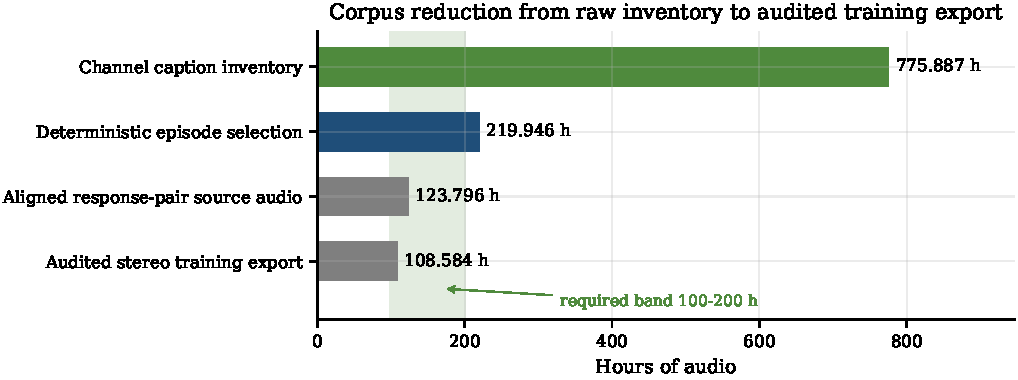
\includegraphics[width=0.95\textwidth]{figs/corpus_funnel.pdf}
\caption{کاهش تدریجی مقدار صوت از موجودی زیرنویس کانال‌ها تا خروجی استریوی
         ممیزی‌شده آموزش. نوار روشن، بازه \N{100} تا \N{200} ساعت مورد نظر
         تعریف پروژه را نشان می‌دهد.}
\label{fig:corpus}
\end{figure}

\section{معماری سامانه آبشاری}
\label{sec:cascade}

سامانه تحویل‌شده پروژه یک زنجیره آبشاری است که کنترل تمام‌دوطرفه روی آن
سوار شده است. \mbox{شکل~\ref{fig:arch}} این معماری را نشان می‌دهد.

\begin{figure}[ht]
\centering
\begin{latin}
\scalebox{0.95}{%
\begin{tikzpicture}[
  box/.style={draw,rounded corners=2pt,align=center,font=\scriptsize,
              minimum height=9mm,inner sep=3pt,text width=24mm},
  client/.style={box,fill=black!5},
  lbl/.style={font=\scriptsize,inner sep=1.5pt,fill=white},
  ar/.style={-{Latex[length=1.8mm]},thin},
  dashar/.style={ar,dashed}
]
% ---- client (left) ----
\node[client] (mic) at (0,0) {continuous mic\\16 kHz PCM16};

% ---- duplex control path (upper row) ----
\node[box] (feat) at (3.1,0)   {rolling features\\energy / F0 / MFCC};
\node[box] (det)  at (6.2,0)   {GBDT barge-in\\classifier};
\node[box] (ctl)  at (9.3,0)   {playback\\controller};

% ---- response chain (lower row) ----
\node[box] (asr)  at (3.1,-2.3) {NeMo Persian\\ASR};
\node[box] (llm)  at (6.2,-2.3) {Qwen3-4B\\prompt-v2};
\node[box] (tts)  at (9.3,-2.3) {Piper Persian\\TTS};

% ---- client sink (right) ----
\node[client] (spk) at (12.4,-1.15) {browser audio\\source};

\draw[ar] (mic)  -- (feat);
\draw[ar] (feat) -- (det);
\draw[ar] (det)  -- (ctl);
\draw[ar] (asr)  -- (llm);
\draw[ar] (llm)  -- (tts);

% end of speech hands the captured turn to the response chain
\draw[ar] (mic.south) |- (asr.west)
      node[lbl,pos=0.18] {end of speech};

% synthesised reply is scheduled by the browser
\draw[ar] (tts.east) -- (spk.south west);

% accepted barge-in stops the active source
\draw[ar] (ctl.east) -- (spk.north west)
      node[lbl,pos=0.55] {stop source};

% retained pre-roll is routed between the two rows into the ASR turn
\draw[dashar] (ctl.south) -- ++(0,-0.50) -| (asr.north)
      node[lbl,pos=0.42] {450 ms pre-roll to next turn};
\end{tikzpicture}}
\end{latin}
\caption{معماری سامانه تحویل‌شده. ردیف بالا مسیر کنترل تمام‌دوطرفه و ردیف
         پایین زنجیره تولید پاسخ است. پیکان نقطه‌چین، انتقال پیش‌بافر
         میکروفون به نوبت بعدی را نشان می‌دهد.}
\label{fig:arch}
\end{figure}

\subsection{بازشناسی گفتار}

جریان صوتی نوبت کاربر به سرویس بازشناسی گفتار فارسی فرستاده می‌شود. این
سرویس یک مدل ترکیبی \en{RNNT-CTC} از خانواده \en{Conformer} است که
به‌صورت محلی و روی رابط شبکه حلقه بازگشتی اجرا می‌شود. متن بازگشتی از
هنجارساز قطعی متن فارسی می‌گذرد تا شکل نویسه‌ها و نیم‌فاصله‌ها یکسان شود.

نکته‌ای که در ممیزی مهم شد، «انتخاب کانال ورودی» است. پرونده‌های
مجموعه داده استریو‌اند و کانال صفر گفتار دستیار و کانال یک گفتار کاربر
است. یک پنل توسعه پیشین به‌اشتباه کانال صفر را به بازشناسی داده بود، یعنی
عملاً صدای بازسازی‌شده دستیار را رونویسی می‌کرد. این اشکال پیش از اجرای هر
ردیف اعتبارسنجی شناسایی و اصلاح شد و پروتکل نهایی، استفاده از کانال یک
«ممیزی‌شده» را الزامی می‌کند.

\subsection{تولید پاسخ متنی}

پاسخ متنی با مدل \en{Qwen3-4B-Instruct-2507} از خانواده
\en{Qwen3}~\cite{qwen2025qwen3} تولید می‌شود. مدل به‌صورت
محلی و از یک درخت پرونده با درهم‌سازی تأییدشده بارگذاری می‌گردد، و
بازنگری مدل و درهم‌سازی درخت در مصنوع نتیجه ثبت می‌شود تا ادعای «مدل دقیقاً
همین بود» قابل ممیزی باشد.

پرامپت سامانه «قفل‌شده» است: متن آن پیش از اجرای ارزیابی تثبیت و
درهم‌سازی آن ثبت شده است. نسخه دوم این پرامپت که در ارزیابی نهایی به کار
رفت، سه قید را به مدل تحمیل می‌کند: پاسخ باید به فارسی باشد، باید کوتاه و
گفتاری باشد، و باید به آخرین اظهار کاربر پاسخ دهد و نه به کل متن رونویسی
شده.

روی خروجی مدل دو نگهبان اعمال می‌شود. نخست یک «قید خط فارسی»: اگر سهم
نویسه‌های فارسی در پاسخ از یک آستانه کمتر باشد، یک تلاش تولید دوباره با
پرامپت تأکیدی انجام می‌گیرد. دوم یک «کران تلاش»: شمار تلاش‌های تولید
حداکثر دو است. اگر هر دو تلاش شکست بخورد، یک پاسخ جایگزین قاعده‌محور تولید
می‌شود. شمار ردیف‌هایی که به این پاسخ جایگزین رسیده‌اند، یکی از شروط پذیرش
ارزیابی است.

پاسخ‌گوی متنی سامانه تحویل‌شده، همان \en{Qwen3-4B-Instruct-2507} با پرامپت
\en{v2} است. پنل مکانیکی نه‌ردیفی اعتبارسنجی و سنجه بازبازشناسی
فصل~\ref{ch:results} اما روی زنجیره پیش از این ارتقا اجرا شده‌اند، یعنی با
پاسخ‌گوی \en{Qwen2.5-0.5B-Instruct} (بازنگری
\en{7ae557604adf67be50417f59c2c2f167def9a775}). آن پنل پس از ارتقا دوباره
اجرا نشد. آزمون معنایی \N{40} ردیفی روی پاسخ‌گوی \en{Qwen3-4B} است و داور آن
مدل هم‌خانواده \en{Qwen3.8-27B-FP8} است
(بازنگری \en{017b9c7af6b5689d5dd426a76e0bc077eb5ca20a})؛ بنابراین کیفیت
معنایی گزارش‌شده، سنجه خودکار هم‌خانواده است و نه اثبات مکانیکی زنجیره
چهارمیلیاردپارامتری روی همان نُه ردیف.

\subsection{تولید گفتار}

متن پاسخ با موتور \en{Piper} و مدل صوتی فارسی به موج صوتی تبدیل می‌شود.
یک مسیر جایگزین مبتنی بر ترکیب فورمانتی نیز پیاده شده است که تنها در
نبود مدل صوتی و برای آزمون‌های نرم‌افزاری به کار می‌رود؛ در همه ردیف‌های
ارزیابی، شرط پذیرش این است که موتور واقعاً \en{Piper} بوده باشد. صوت خروجی
از نظر متناهی‌بودن مقادیر، طول کمینه، هنجارسازی دامنه و
«غیرساکت بودن» با معیار ریشه میانگین مربعات بررسی می‌شود.

\section{ماژول تشخیص وقفه و بستر تمام‌دوطرفه}
\label{sec:bargein}

\subsection{استخراج ویژگی و طبقه‌بند}

ویژگی‌های توضیح‌داده‌شده در بخش~\ref{sec:features} به‌صورت غلتان روی جریان
میکروفون محاسبه می‌شوند: فریم \N{20} میلی‌ثانیه، پنجره متن
\N{400} میلی‌ثانیه، \N{13} ضریب \en{MFCC} با دلتاهای متناظر، بسامد پایه با
روش \en{YIN} در بازه \N{60} تا \N{400} هرتز، انرژی لگاریتمی و نرخ گذر از
صفر. برای هر بعد، سه آماره میانگین، انحراف معیار و بیشینه روی پنجره
محاسبه و به هم پیوند داده می‌شود.

بردار حاصل، پس از هنجارسازی، به یک طبقه‌بند تقویت گرادیانی داده می‌شود
(بخش~\ref{sec:gbdt}) با \N{200} درخت، عمق بیشینه \N{4}، نرخ یادگیری
\N{0.08} و کمینه \N{8} نمونه در برگ. کلاس‌های هدف عبارت‌اند از نبود رخداد،
وقفه، بازخورد کلامی و نویز. برای مقایسه، یک «خط پایه» مبتنی بر
آستانه‌گذاری انرژی و نرخ گذر از صفر نیز پیاده شده است.

\subsection{کنترل پخش و پیوستگی نوبت}

یک مؤلفه «کنترل‌گر پخش» مالک مسیر تصمیم است. این مؤلفه وضعیت پخش را
نگه می‌دارد، در هنگام پخش قطعه‌های میکروفون را به آشکارساز می‌دهد و در صورت
مثبت‌شدن تصمیم، رویداد توقف را به کارخواه می‌فرستد و زمان آغاز آوایی تا
تأیید توقف را ثبت می‌کند.

سازوکاری که برای تجربه کاربری تعیین‌کننده است، «پیش‌بافر» است. آشکارساز
همیشه \N{450} میلی‌ثانیه آخر جریان میکروفون را در یک بافر غلتان نگه
می‌دارد. هنگامی که وقفه پذیرفته می‌شود، این پیش‌بافر دور ریخته نمی‌شود، بلکه
با صوتی که پس از آن دریافت می‌گردد به هم پیوند می‌خورد و ورودی نوبت بعدی
را می‌سازد. بدون این سازوکار، آغاز جمله کاربر از دست می‌رفت و او ناچار
می‌شد جمله را از نو بگوید.

بستر انتقال، یک اتصال \en{WebSocket} است که جریان \en{PCM16} پیوسته را از
مرورگر می‌گیرد و رویدادهای کنترلی را در هر دو جهت رد‌و‌بدل می‌کند. آزمون‌های
بازگشتی خودکار این بستر، پیوستگی پیش‌بافر و صوت پس از آن، دریافت تأیید
توقف از کارخواه، لغو نوبت، اتصال مجدد، جداسازی وضعیت نشست‌ها، بازیابی از
خطای تولید و حالت نگه‌داری فقط‌سنجه بدون ذخیره پرونده صوتی را پوشش
می‌دهند.

\مرزادعا{این آزمون‌ها پیوستگی را در «سطح انتقال» اثبات می‌کنند. توقف
منبع صوت در یک مرورگر واقعی با میکروفون فیزیکی اندازه‌گیری نشده است و
بنابراین سنجه‌های رسمی $T_{\text{first\_audio}}$ و
$T_{\text{barge\_in}}$ در این نوشتار گزارش نمی‌شوند.}

\subsection{ارزیابی روی داده ضبط‌شده}

برای سنجش آشکارساز روی صوت واقعی، رخدادهای تعاملی از مرزهای تفکیک گوینده
در پنجره‌های مجموعه داده کشف شدند. از \N{1,730} رخداد کشف‌شده،
\N{1,048} رخداد با شرط تعادل کلاس‌ها انتخاب و بر پایه نشست به سه بخش
تقسیم شد. آستانه تصمیم «تنها» روی نشست‌های اعتبارسنجی و با معیار
ازپیش‌تعریف‌شده انتخاب گردید و سپس یک‌بار روی نشست‌های آزمون اعمال شد.

\section{طراحی آزمایش‌های مسیر مستقیم}
\label{sec:direct}

\subsection{هدف آموزشی و شرط پذیرش}

مسیر مستقیم، تطبیق کم‌پارامتر مدل \en{Moshika} با آموزش‌دهنده رسمی آن است.
داده ورودی، همان پرونده‌های استریوی بخش~\ref{sec:data} است: کانال صفر
گفتار دستیار بازسازی‌شده و کانال یک گفتار کاربر، همراه با هم‌ترازی متنی
که سازوکار «تک‌گویی درونی» به آن نیاز دارد. زیان کل، ترکیب وزن‌دار زیان
نشانه‌های متنی و زیان نشانه‌های صوتی هر کتاب رمز است.

تصمیم روشمند مرکزی این بخش، تعریف یک «شرط پذیرش زمان اجرا» پیش از
آغاز آموزش بود. برای هر چک‌پوینت نامزد، آداپتر در سرور جویباری رسمی مدل
بارگذاری می‌شود، نه در یک اسکریپت محلی، و برای هر یک از ۹ ردیف ورودی از
پیش تعیین‌شده باید هم‌زمان چند شرط برقرار باشد: مدل باید متن تولید کند،
باید گفتار غیرساکت تولید کند، و متن تولیدی باید از قید خط فارسی بگذرد. یک
چک‌پوینت تنها در صورتی «واجد شرایط» است که هر \N{9} ردیف را با موفقیت
بگذراند.

این شرط سخت‌گیرانه است و به‌طور عمدی چنین طراحی شده. تجربه نسخه نخست نشان
داد که چک‌پوینت‌هایی با کمترین زیان اعتبارسنجی، در تولید خودرگرسیو صوت
تقریباً ساکت و بدون متن می‌دهند. اگر انتخاب چک‌پوینت تنها بر زیان استوار
بود، همان مصنوع بی‌فایده به‌عنوان «مدل فارسی» گزارش می‌شد.

\subsection{شش نسل آزمایشی}

آزمایش‌ها به‌صورت زنجیره‌ای از فرضیه‌های قابل ابطال طراحی شدند و در هر نسل
تلاش شد «تنها یک عامل» تغییر کند. جدول~\ref{tab:moshi-design} این
طراحی را خلاصه می‌کند.

\begin{table}[ht]
\centering
\caption{طراحی شش نسل آزمایشی مسیر مستقیم و فرضیه‌ای که هر نسل آزمود}
\label{tab:moshi-design}
\small
\begin{tabular}{lL{3.1cm}L{4.4cm}c}
\toprule
\textbf{نسخه} & \textbf{عامل تغییر‌یافته} & \textbf{فرضیه آزمون‌شده} &
\textbf{رتبه} \\
\midrule
\en{v1} & پیکربندی پایه، پنجره \N{20} ثانیه، آموزش همه درج‌گرها &
مدل با داده کافی، گفتار فارسی می‌آموزد & \N{64} \\
\en{v2} & پنجره متن به \N{100} ثانیه &
پنجره کوتاه، آغاز پاسخ را در بافت نمی‌گنجاند & \N{64} \\
\en{v3} & انجماد همه درج‌گرها و رتبه بالاتر &
آموزش درج‌گرها بازنمایی پایه را تخریب می‌کند & \N{128} \\
\en{v4} & آموزش تنها دو درج‌گر متنی &
تنها فضای متنی فارسی نیاز به تطبیق دارد & \N{128} \\
\en{v5} & ضریب زیان کتاب رمز نخست از \N{100} به \N{10} &
وزن زیاد کتاب رمز معنایی، یادگیری آوایی را خفه می‌کند & \N{128} \\
\en{v6.2} & آزمون ظرفیت درون‌نمونه با حذف تصادفی ورودی متنی و پنجره \N{12} ثانیه &
مدل ظرفیت یادگیری دارد و مشکل، اریبی مواجهه است & \N{64} \\
\bottomrule
\end{tabular}
\end{table}

سه نسخه نخست، مسیر متعارف تنظیم فراپارامتر را می‌پیمایند. نسخه‌های چهارم و
پنجم، فرضیه‌های دقیق‌تری را می‌آزمایند که از تحلیل شکست نسخه‌های پیشین
برآمده‌اند: اگر مشکل، نبود بازنمایی متنی فارسی است، آموزش گزینشی تنها دو
درج‌گر متنی باید کافی باشد؛ و اگر مشکل، غلبه زیان معنایی بر زیان آوایی
است، کاهش ضریب کتاب رمز نخست باید آن را برطرف کند.

نسخه ششم، طراحی متفاوتی دارد و به‌عمد یک «آزمون ابطال» است. در این
نسخه، مدل روی تنها \N{32} نمونه و با پنجره متن \N{12} ثانیه آموزش می‌بیند و روی «همان» \N{32}
نمونه ارزیابی می‌شود. هدف، سنجش تعمیم نیست، بلکه پاسخ به یک پرسش دو‌گزینه‌ای
است: آیا این آداپتر «ظرفیت» یادگیری هدف را دارد یا نه؟ اگر مدل
نتواند حتی روی داده آموزشی خودش زیان را به‌قدر کافی کاهش دهد، مشکل در
ظرفیت است؛ اگر بتواند اما در تولید خودرگرسیو شکست بخورد، مشکل در
اریبی مواجهه است (بخش~\ref{sec:exposure-bias}). نسخه \en{v6.2} همچنین
«حذف تصادفی زمان‌بندی‌شده ورودی متنی» را اضافه می‌کند: سهم نشانه‌های
متنی مرجع که در آموزش پنهان می‌شوند به‌تدریج از \N{0.25} به \N{0.75}
افزایش می‌یابد تا مدل بیاموزد بر پیش‌بینی خودش تکیه کند.

\section{روش کاری شواهد‌محور}
\label{sec:evidence-first}

بخش بزرگی از سهم روشمند این پروژه، در چگونگی «گزارش» نتایج است.
تجربه تلاش اولیه (\mbox{بخش~\ref{sec:early-attempt}}) نشان داد که یک مصنوع
می‌تواند زیان کاهنده و ظاهر موفق داشته باشد و در همان حال هیچ ادعای
معناداری را پشتیبانی نکند. برای پرهیز از تکرار این وضعیت، پنج قاعده
عملیاتی تعریف و در کد اعمال شد.

\paragraph{یک. تعریف پیشینی پروتکل.} برای هر ارزیابی، یک سند پروتکل شامل
شاخص دقیق ردیف‌های آزمون، آستانه‌های پذیرش، بازنگری مدل‌ها و درهم‌سازی
پرونده‌ها، پیش از اجرا نوشته و در مخزن ثبت می‌شود. آستانه پذیرش پس از
مشاهده نتیجه ساخته نمی‌شود.

\paragraph{دو. تفکیک مرحله صلاحیت از آزمون نهایی.} ارزیابی معنایی دو‌مرحله‌ای
است. نخست یک مرحله صلاحیت روی شمار کوچکی از ردیف‌های اعتبارسنجی اجرا
می‌شود. تنها در صورت عبور کامل از این مرحله، آزمون نهایی روی ردیف‌های
آزمون «یک‌بار» باز می‌شود. این طراحی از انتخاب پس از مشاهده نتیجه
جلوگیری می‌کند. داور این ارزیابی، مدل \en{Qwen3.8-27B-FP8} با بازنگری
\en{017b9c7af6b5689d5dd426a76e0bc077eb5ca20a}، دمای صفر، ترتیب بازوی
دوسوکور و دو تکرار در هر ردیف است. چون داور و نامزد از یک خانواده‌اند،
نتیجه در کلاس «تقریب خودکار هم‌خانواده» می‌ماند و نیازمندی تعریف پروژه را
اثبات نمی‌کند.

\paragraph{سه. مصنوعات یک‌بار‌نوشت.} هر نتیجه نهایی در یک پرونده ساختارمند
ثبت می‌شود که شامل مقادیر اندازه‌گیری‌شده، وضعیت هر شرط پذیرش،
درهم‌سازی‌های ورودی، مشخصات سخت‌افزار و یک فهرست صریح محدودیت‌ها است. این
پرونده بازنویسی نمی‌شود.

\paragraph{چهار. کلاس‌بندی شواهد.} هر اندازه‌گیری با یک «کلاس شواهد»
برچسب می‌خورد. جدول~\ref{tab:evidence-classes} این کلاس‌ها را تعریف
می‌کند. قاعده بنیادی آن است که تنها کلاس رسمی می‌تواند برآورده‌شدن یک
نیازمندی تعریف پروژه را اثبات کند.

\begin{table}[ht]
\centering
\caption{کلاس‌های شواهد و توان ادعای هر کلاس}
\label{tab:evidence-classes}
\small
\begin{tabular}{L{3.3cm}L{5.4cm}c}
\toprule
\textbf{کلاس شواهد} & \textbf{شرایط لازم} & \textbf{اثبات نیازمندی} \\
\midrule
رسمی سرتاسری & نشست زنده با رضایت کاربر، تأیید پخش از سوی کارخواه،
میکروفون واقعی و سخت‌افزار واجد شرایط & مجاز \\
زنده غیر‌رسمی & همان پروتکل، اما سخت‌افزار یا شرایط مطالعه واجد شرایط نیست
& غیر‌مجاز \\
مؤلفه سمت سرور & زمان‌سنجی تولید یا آشکارساز، بدون اثبات رفتار شنیدنی
کارخواه & غیر‌مجاز \\
تقریب مصنوعی & صوت تولیدشده یا رخداد شبیه‌سازی‌شده & تنها آزمون بازگشتی \\
تقریب خودکار هم‌خانواده & داوری با مدل زبانی از خانواده نامزد & غیر‌مجاز \\
\bottomrule
\end{tabular}
\end{table}

\paragraph{پنج. تجمیع شکست‌بسته.} یک مؤلفه تجمیع‌کننده، همه مصنوعات نتیجه
را می‌خواند و وضعیت کلی پروژه را می‌سازد. این مؤلفه «شکست‌بسته» است:
اگر مصنوع پشتیبان یک شرط وجود نداشته باشد، یا درهم‌سازی آن با ورودی
مورد انتظار نخواند، یا کلاس شواهد آن پایین‌تر از حد لازم باشد، آن شرط
«ناموفق» گزارش می‌شود و نه «نامعلوم». همچنین این مؤلفه صریحاً مانع
از ارتقای یک تقریب به شواهد رسمی می‌شود.

پیامد این روش کاری آن است که وضعیت شواهد هر شرط، همان‌طور که در
فصل~\ref{ch:results} گزارش می‌شود، مستقل از آمادگی گزارش برای ارائه و
داوری بیان شود. نتیجه نهایی، تفکیک روشن آنچه ساخته شده از آنچه با شواهد
رسمی اثبات شده است.

\section{پیاده‌سازی و بازتولیدپذیری}
\label{sec:impl}

کد پروژه در یک بسته پایتون با رابط خط فرمان یکپارچه سازمان یافته است که
هر مرحله زنجیره داده، آموزش، ارزیابی و سرویس‌دهی را به‌صورت یک زیرفرمان
مستقل ارائه می‌کند. پیاده‌سازی مدل‌ها بر \en{PyTorch}~\cite{paszke2019pytorch}
و کتابخانه \en{Transformers}~\cite{wolf2020transformers} استوار است. دو محیط مجازی جداگانه نگه داشته می‌شود: یکی برای
سامانه اصلی و یکی برای پشته مسیر مستقیم که وابستگی‌های سخت‌گیرانه‌تری
دارد.

سه سازوکار، بازتولیدپذیری را پشتیبانی می‌کنند. نخست، یک پرونده قفل
«مخازن بالادستی» که برای هر مدل و مخزن بیرونی، بازنگری دقیق و
درهم‌سازی وزن‌ها را ثبت می‌کند. دوم، بذر تصادفی ثابت برای هر آزمایش که در
مصنوع نتیجه گزارش می‌شود. سوم، مجموعه آزمون خودکار به همراه یکپارچه‌سازی
پیوسته که در آن، بررسی سبک کد، بررسی نوع، ممیزی آسیب‌پذیری وابستگی‌ها،
ممیزی مصنوعات ثبت‌شده و پوشش آزمون اجرا می‌شود.

فرمان‌های بازتولید هر مرحله در پیوست~\ref{sec:appendix-commands} فهرست شده‌اند.
